\documentclass[11pt]{article}
\usepackage{graphicx,bm,amssymb,amsmath,amsthm}
% timo macros...
\newcommand{\bx}{\textbf{x}}
\newcommand{\by}{\textbf{y}}
\newcommand{\bs}{\textbf{s}}

% alex macros...
\newcommand{\bi}{\begin{itemize}}
\newcommand{\ei}{\end{itemize}}
\newcommand{\ben}{\begin{enumerate}}
\newcommand{\een}{\end{enumerate}}
\newcommand{\be}{\begin{equation}}
\newcommand{\ee}{\end{equation}}
\newcommand{\bea}{\begin{eqnarray}}
\newcommand{\eea}{\end{eqnarray}}
\newcommand{\bc}{\begin{center}}
\newcommand{\ec}{\end{center}}
\newcommand{\bfi}{\begin{figure}}
\newcommand{\efi}{\end{figure}}
\newcommand{\ca}[2]{\caption{#1 \label{#2}}}
\newcommand{\ig}[2]{\includegraphics[#1]{#2}}
\newcommand{\spl}[2]{\left\{\begin{array}{ll}#1\\#2\end{array}\right.}
\newcommand{\ie}{{\it i.e.\ }}
\newcommand{\eg}{{\it e.g.\ }}
\newcommand{\pd}[2]{\frac{\partial #1}{\partial #2}}
\newcommand{\pdc}[3]{\left. \frac{\partial #1}{\partial #2}\right|_{#3}}
\newcommand{\infint}{\int_{-\infty}^{\infty} \!\!}      % infinite integral
\newcommand{\tbox}[1]{{\mbox{\tiny #1}}}
\newcommand{\mbf}[1]{{\bm #1}}           % requires bm package
\newcommand{\pO}{{\partial\Omega}}
\newcommand{\uN}{u^{(N)}}
\newcommand{\emach}{\epsilon_\tbox{mach}}
%\newcommand{\crk}{C_{s}} %C_{R,k}         % const for exponential s(m) bnd
\newcommand{\bmp}[1]{\begin{minipage}{#1}}
\newcommand{\emp}{\end{minipage}}
\newcommand{\re}{\mbox{Re}\,}
\newcommand{\im}{\mbox{Im}\,}

\newtheorem{thm}{Theorem}
\newtheorem{cnj}{Conjecture}
\newtheorem{lem}{Lemma}[thm]
\newtheorem{cor}{Corollary}[thm]

\newtheorem{rmk}[thm]{Remark}
\newtheorem{pro}[thm]{Proposition}
%\newtheorem{cnj}[thm]{Conjecture}
%\newtheorem{lemma}[thm]{Lemma}

\newcommand{\bp}{{\bf Proof:\ }}   % {\begin{proof}}
\newcommand{\ep}{\hfill $\square$ \vspace{1ex} \\} % {\end{proof}}
% note elsart ones horrible: \pr and \endpr
\newcommand{\bmal}{{\bm \alpha}}             % bold alpha
\newcommand{\splt}[2]{$\left\{\begin{array}{l}\mbox{#1}\\\mbox{#2}\end{array}\ri
ght.$}
\newcommand{\lo}{{L^2(\Omega)}}
\newcommand{\lpo}{{L^2(\pO)}}
\newcommand{\cu}{\tilde{u}}            % symbol for continuation of u
\newcommand{\cOmega}{\tilde{\Omega}}   % symbol for domain to be continued into
\newcommand{\dmax}{D_\tbox{max}}       % max dist in splane_charge_curve

% spacers...
\newcommand{\tw}{\textwidth}
\newcommand{\vg}{\vspace{2ex}}

% brand names... the problem with putting a trailing space here is that then
% punctuation following the word cannot be correct. To use these with correct
% trailing space, use as \mpspack\ or \matlab\ or with ending period, \matlab.
\newcommand{\mpspack}{{\tt MPSpack}}            % name of this package
\newcommand{\matlab}{{M{\small ATLAB}}}            % name of MATLAB

% code formatting... (nearly ok, gets multiple-line padding wrong)
\newcommand{\co}[1]{\vspace{.5ex}
\\
\mbox{}\hspace{5ex}\begin{minipage}{\textwidth}{\tt #1}\end{minipage}%
\vspace{.5ex}%
\\}



\begin{document}
\title{\mpspack\ tutorial}
\author{Alex Barnett\footnote{Department of Mathematics, Dartmouth College,
Hanover, NH, 03755, USA}
\ and
Timo Betcke\footnote{Department of Mathematics,
University of Reading, Berkshire, RG6 6AX, UK}}
\date{\today}   % how pipe from getrevisionnumber + 1?

\maketitle
\begin{abstract}
This tutorial shows how a variety of two-dimensional Laplace and Helmholtz
boundary-value and eigenvalue problems
may be numerically solved simply and accurately with the \mpspack\ toolbox
for \matlab. We assume basic familiarity with \matlab\
and with partial differential equations.
%concept of particular-solution type numerical methods is assumed.
\end{abstract}

\setcounter{tocdepth}{2}
\tableofcontents

\section{About this tutorial}

This tutorial is designed for `bottom-up' learning of the features
of \mpspack, i.e.\ by progressing through simple examples.
In that sense it complements the user manual which describes
the theoretical framework in broad strokes and therefore could
be considered `top-down'.
We will skip most of the mathematics behind the techniques,
focusing on computing and plotting useful PDE solutions.
We hope you will try each command as you read!

Throughout we will identify the plane $\mathbb{R}^2$ with the complex
plane $\mathbb{C}$, by the usual map $z=x+iy$. In other words
$(2,3)$ and $2+3i$ represent the same point.
We use {\tt teletype} font to designate commands that may be typed
at the \matlab\ prompt.
You may get help on any \mpspack\ command by typing {\tt help command}.
All the code examples in this document, including code to generate the
figures, is found in the {\tt examples/} directory.
The codes for Sections \ref{s:lap}--\ref{s:qpsc} are named
\verb@tut_*.m@ according to the section names in {\tt tutorial.tex}.

Computation times are reported for a single core (mostly what MATLAB
uses) of an Intel laptop CPU (either Core Duo from 2006, or i7-3720QM
from 2012).

\bfi % ffffffffffffffffffffffffffffffffffffffffffffffffffffffffffffffffffffff
a)\raisebox{-0.3\textwidth}{\ig{height=0.35\textwidth}{seg.eps}}
b)\raisebox{-0.3\textwidth}{\ig{height=0.35\textwidth}{dom.eps}}
\ca{a) circular closed segment, b) unit disc domain.
Both have a periodic trapezoidal quadrature rule
with $M=20$ quadrature points}{f:sd}
\efi

% ----------------------------------------------------------------------------
\section{Solving Laplace's equation in a disc}
\label{s:lap}

We start by setting up a domain in $\mathbb{R}^2$.
% in which a PDE will be solved.
Domains are built from segments which define their boundary.
To make the unit disc domain,
we first need a circle segment with center
0, radius 1, and angle range
$[0,2\pi)$, as follows,
\co{s = segment([], [0 1 0 2*pi])}
The object {\tt s} is indeed a circular segment, as we may check by
typing {\tt s.plot}, producing Fig.~\ref{f:sd}a.
%or by examining its contents by typing {\tt s}.
All segments have a {\em sense}, i.e.\ direction of travel:
for this segment it is counter-clockwise, as shown by the
downwards-pointing
arrow symbol overlayed onto the segment at about 9 o'clock.%
  \footnote{In fact, segments are parametrized internally as function $z(t)$
    of a real variable $t\in[0,1]$, and the sense is the direction of
    increasing $t$. Segment {\tt s} stores this function as {\tt s.Z}.}
Notice also normal vectors (short `hairs') pointing outwards
at each boundary point; our definition is that
normals on a segment always point to the {\em right} when traversing the
sense of the segment.

We create the domain interior to this segment with
\co{d = domain(s, +1)}
where the second argument (here $+1$, the only other option being $-1$)
specifies that the domain is to the `standard' side of the segment, which
we take to be such that the normals point {\em away from} the domain.
That is, with $+1$ the domain lies to the {\em left} of the segment
when traversed in its correct sense (with $-1$ the domain
would lie to the right of the segment.)
Typing {\tt d.plot} produces%
  \footnote{There are extra plotting options and features that
    are described in documentation such as {\tt help domain.plot}.
    E.g.\ in this figure a grid of points interior to the domain has been
    included, achieved with {\tt opts.gridinside=0.05; d.plot(opts);}
    %TODO: demo switch off corner fan.
  }
Fig.~\ref{f:sd}b.
Note that perimeter and area are automatically
labelled (these are only rough approximations intended for sanity checks).

\bfi % ffffffffffffffffffffffffffffffffffffffffffffffffffffffffffffffffffffff
a)\raisebox{-0.3\textwidth}{\ig{height=0.35\textwidth}{u.eps}}
b)\raisebox{-0.3\textwidth}{\ig{height=0.35\textwidth}{uerr.eps}}
\ca{a) Numerical solution field $u$, b) pointwise error $u-f$,
for Laplace's equation in the unit disc with $M=20$ quadrature points
and 8th-order harmonic polynomials.}{f:u}
\efi

Laplace's equation $\Delta u = 0$ is Helmholtz's equation with wavenumber
zero, which we set for this domain with,
\co{d.k = 0;}
Our philosophy is
to approximate the solution in the domain by a linear combination of
{\em basis functions}, each defined over the whole domain.
%We have to choose how many to use, i.e.\ the
%{\em order} of approximation.
We choose 8th-order harmonic polynomials
$u(z) = \sum_{n=0}^{8} c_n \,\mbox{Re}\,z^n +
\sum_{n=1}^{8} c_{-n}\,\mbox{Im}\,z^n$, where $\mbf{c}:=\{c_n\}_{n=-8}^{8}
\in\mathbb{R}^{17}$
is a coefficient vector, based at the origin 0,
%i.e.\ the sets $\{\mbox{Re } z^n\}_{n=0}^{10}$ and
%$\{\mbox{Im } z^n\}_{n=1}^{10}$,
using the command
\co{d.addregfbbasis(0, 8);}
Let's specify Dirichlet boundary data $f(z) = 
\ln |z-2-3i|$ for
$z$ on the segment%
  \footnote{In other words, $f(x,y) = \ln \sqrt{(x-2)^2+(y-3)^2}$
    for points $(x,y)$ on the boundary.}
by representing this as an anonymous function {\tt f}
and associating it with one side of the segment,
\begin{verbatim}
   f = @(z) log(abs(z-2-3i));
   s.setbc(-1, 'd', [], @(t) f(s.Z(t)));
\end{verbatim}
Note that we needed to pass in a function not of location $z$,
but of the segment parameter $t$;
this was achieved by
wrapping ${\tt f}$ around the parametrization function ${\tt s.Z}$.
The first argument $-1$ expresses that the boundary condition is to be
understood in the limit approaching from the side {\em opposite} the
segment's normal direction, which is where the domain is located.
The second argument {\tt 'd'} specifies that the data is Dirichlet.
 
Finally we use the domain to make a boundary-value
problem object {\tt p},
\co{p = bvp(d);}
and may then solve (in the least-squares sense)
a linear system for the coefficients
\co{p.solvecoeffs;}
If it is needed, {\tt p.co} now contains the coefficients vector $\mbf{c}$.
To evaluate and plot the solution we simply use,
\co{p.showsolution;}
The software chose an appropriate grid covering the domain
(points outside the domain are made transparent), giving Fig.~\ref{f:u}a.

\bfi % ffffffffffffffffffffffffffffffffffffffffffffffffffffffffffffffffffffff
a)\raisebox{-0.3\textwidth}{\ig{height=0.35\textwidth}{N.eps}}
b)\raisebox{-0.3\textwidth}{\ig{height=0.35\textwidth}{radfunc.eps}}
\ca{a) Convergence of boundary error $L^2$ norm for harmonic
polynomials for Laplace equation
in the unit disc, b) solution error for same boundary data $f$
in a smooth star-shaped `trefoil' domain (normals also shown).}{f:conv}
\efi

% ----------------------------------------------------------------------------
\section{Accuracy, convergence, and smooth domains}
\label{s:conv}

How accurate was our numerical solution $u$? One measure is the
$L^2$ error on the boundary, and is estimated by
\co{p.bcresidualnorm}
which returns $2.09 \times 10^{-6}$.
However, since the function $f(z)$ is already harmonic in the domain,
it is in fact the unique solution, and we may plot the
pointwise error in $u$ by passing in the analytic solution as an option,
\co{opts.comparefunc = f; p.showsolution(opts);}
giving Fig.~\ref{f:u}b. Note that the color scale is $10^{-8}$.

In the above, boundary integrals were approximated using the default of
$M=20$ quadrature points, barely adequate given the
oscillatory error function in Fig.~\ref{f:u}b.
$M$ may be easily changed either by specifying
a non-empty first argument in the {\tt segment} constructor above, or
for an existing segment as follows,
\co{s.requadrature(50); p.solvecoeffs; p.bcresidualnorm}
which now gives $1.98\times 10^{-6}$, not much different than before.
Notice that we did not have to redefine the domain {\tt d} nor
the BVP object {\tt p}.

Exploring the convergence of the boundary error norm with the basis set order
needs a simple loop and figure,
\begin{verbatim}
   for N=1:15
     d.bas{1}.N = N; p.solvecoeffs; r(N) = p.bcresidualnorm;
   end
   figure; semilogy(r, '+-'); xlabel('N'); ylabel('bdry err norm');
\end{verbatim}
As Fig.~\ref{f:conv}a shows, the convergence is exponential.%
  \footnote{Asymptotically, error $\sim e^{-\alpha N}$. In fact the rate is
    $\alpha = \ln \sqrt{13}$, related to the conformal distance to
    the nearest singularity \cite{timothesis}, which here is at $2+3i$.}

Say we want to change the shape of segment {\tt s}, to
a smooth star-shaped `trefoil' domain expressed as by radius $R(\theta) =
1 + 0.3\cos 3\theta$ as a function of angle $0\le \theta< 2\pi$.
This is achieved by passing a 1-by-2
cell array containing the function $R$ and its
derivative $R' = dR/d\theta$ to a variant of the segment constructor,
\begin{verbatim}
   s = segment.radialfunc(50, {@(q) 1 + 0.3*cos(3*q), @(q) -0.9*sin(3*q)});
\end{verbatim}
We again chose $M=50$.
The analytic formula for $R'$ is needed to compute normal derivatives
to high accuracy.

One might ask: has this change to {\tt s} {\em propagated}
to the existing domain
object {\tt d} and BVP object {\tt p}, which both refer to it?
In contrast to the case of quadrature point number $M$ above,
the answer is no:
{\tt s} is overwritten by a newly-constructed object, while
{\tt d} and {\tt p} still contain handles pointing to the {\em old}
{\tt s}.
Furthermore, the fact that the segment had domain {\tt d}
attached to its `minus' or back side has been forgotten, as have the
boundary conditions.
(These segment properties are described in the \mpspack\ user manual.)
We must therefore rerun the code from Sec.~\ref{s:lap}
to construct {\tt d} and {\tt p} afresh, before solving.%
  \footnote{Note that in theory it would be possible to
    change one by one each of the segment properties, {\tt t}, {\tt w},
    {\tt speed}, etc, to define the new segment without changing its identity,
    but this is cumbersome. Similarly, searching and changing
    all references to a segment in the properties of {\tt d} and {\tt p}
    is cumbersome. Neither has been implemented since problem setup time is
    very rapid.}
The result, plotting the pointwise error as before,
is shown by Fig.~\ref{f:conv}b for $N=8$ and $M=50$.

The {\tt radialfunc} constructor above is limited to radial functions
with quadrature equidistant
in angle. Instead you may create a segment from arbitrary
smooth parametrizations $z(t)$ for $t \in[0,1]$, as long as $z'(t)$
is also given. For instance, a closed crescent-shaped analytic segment is
produced by 
\begin{verbatim}
   a = 0.2; b = 0.8; w = @(t) exp(2i*pi*t);
   s = segment(100, {@(t) w(t)-a./(w(t)+b), ...
                     @(t) 2i*pi*w(t).*(1 + a./(w(t) + b).^2)}, 'p');
\end{verbatim}
Note the nested anonymous functions for mathematical clarity.
Note also the new final argument {\tt 'p'} which enforces
periodic quadrature (the constructor doesn't try to guess your preferred rule).
In order to get high-order (or spectral) convergence, it is recommended
that you choose only smooth (or analytic) $z$.
If periodic quadrature is used,
this also applies to the 1-periodic extension of $z$ to the real line.
If $z(1)\neq z(0)$, the ends of the segment will not connect
up, and the domain constructor above will report an error.


% ----------------------------------------------------------------------------
\section{Helmholtz equation, exterior and multiply connected domains}

Changing from the Laplace to Helmholtz equation is as simple
as setting {\tt d.k} to a positive value.
We start a fresh example: a exterior Helmholtz BVP
with Neumann boundary data, and the Sommerfeld radiation
condition \cite{coltonkress}. This has a unique solution.

The simplest unbounded domain is $\mathbb{R}^2$, which is created with
\co{d = domain();}
One may check that its area {\tt d.area} is $\infty$.
Exterior domains can be created by excluding a closed segment, for instance
the trefoil segment introduced above,
\begin{verbatim}
   tref = segment.radialfunc(50, {@(q) 1 + 0.3*cos(3*q), @(q) -0.9*sin(3*q)});
   d = domain([], [], tref, -1);                    % overwrites previous d
\end{verbatim}
Note the choice $-1$ for the direction argument, which states that
the domain lies on the `nonstandard' side of the segment, i.e.\
to the right side as the segment is traversed in its natural sense,
with the segment normals pointing {\em into} the exterior domain.






[TIMO insert mfsbasis, solve exterior smooth domain Helmholtz Dirichlet
BVP. Add your code to examples/tutorial.m]

\vspace{10ex}














\bfi % ffffffffffffffffffffffffffffffffffffffffffffffffffffffffffffffffffffff
a)\raisebox{-0.4\textwidth}{\ig{height=0.45\textwidth}{twoholes.eps}}
b)\raisebox{-0.4\textwidth}{\ig{height=0.45\textwidth}{tri.eps}}
\ca{a) A multiply-connected domain. b) A polygonal domain.}{f:doms}
\efi

A non-simply connected domain may be built by specifying excluded
regions from a simply connected bounded domain. For example,
to remove from an interior trefoil a circular `hole',
\begin{verbatim}
   tref.disconnect;                         % clears any domains from segment
   c = segment([], [0.5 0.4 0 2*pi]);       % new circular segment
   d = domain(tref, 1, c, -1);
\end{verbatim}
Note that segment {\tt tref} had previously
been `linked' to the old domain {\tt d}
at the start of this section, hence the need to `disconnect' it
(or create a fresh segment) before
building new domains from it. 
If the direction signs $+1$ and $-1$ are not correct as above, an
error is reported (check this!)
We may exclude two regions as follows, where the new region is a smaller copy
of the trefoil,
\begin{verbatim}
   tref.disconnect; c.disconnect;
   smtref = tref.scale(0.3);                % create new rescaled copy of tref
   smtref.translate(-0.3+0.4i);             % move the segment smtref
   d = domain(tref, 1, {c smtref}, {-1 -1});
\end{verbatim}
Typing {\tt d.plot} gives Fig.~\ref{f:doms}a. Notice that
the domain's boundary is the union of three segments. They are labeled
1, 2, and 3, showing the order in which segment handles
are stored internally in the domain object {\tt d.seg}.
The convention for plotting domains is that the normals
are those of the domain, rather than the normal intrinsic to each segment.
The figure shows all normals pointing away from the domain, as it should.
Similarly, the arrow directions are modified by the signs $(1,-1,-1)$ that
were passed in, so that, following the arrows the domain always lies to
the {\em left}. (The black semicircles will be explained in the next section.)


[MAYBE add mfsbasis example here with three src curves one for each segment?]

\vspace{10ex}





% ----------------------------------------------------------------------------
\section{Polygons, corners, and corner-adapted bases}
\label{s:poly}

So far each disconnected boundary piece of the domain
has been a single segment connected to itself head-to-tail.
More generally, a {\em list} of segments may be used to create 
these closed boundary pieces, as long as the last in the list
connects back to the starting point of the first.
For instance, a triangle is built from sending a list of
three line segments to the domain command;
this list may conveniently be made with a polygon constructor,
\begin{verbatim}
   s = segment.polyseglist([], [1, 1i, exp(4i*pi/3)]);
   tri = domain(s, 1);
\end{verbatim}
Since {\tt s} is a 1-by-3 array of (handles to) segments,
the 2nd argument is automatically vectorized to {\tt [1 1 1]}.
Each of the segments could have been made separately, e.g.\ the first by
\co{s(1) = segment([], [1 1i]);}
Fig.~\ref{f:doms}b shows {\tt tri.plot} output for this domain.%
  \footnote{Notice that periodic quadrature would now be inappropriate:
    in fact $M=20$ point Clenshaw-Curtis is used by default for open
    segments}

Let's discuss corners: their angles are indicated by the solid black
`fans' in the plot (before now these have had angle $\pi$, hence semicircles).
A black fan at the junction of two segments indicates that a corner
linkage was made (warnings will be given if any segment ends are left
dangling), and shows the angle range pointing {\em into} the domain.
%The data is stored in the domain properties as {\tt tri.
%and their start and end angles

Segment lists may also be sent to the excluded arguments of the
domain constructor, for instance to create the domain exterior
to the triangle,
\co{exttri = domain([], [], s(end:-1:1), -1);}
where it was important to reverse the order of the segment list,
since each was 
or to create the domain exterior to two nearby triangles,
\begin{verbatim}
   ss = s.translate(2);
   exttwotri = domain([], [], {s(end:-1:1), ss(end:-1:1)}, {-1, -1});
\end{verbatim}
We remind the reader that to create the above domains
using the existing segment array {\tt s}, each time a {\tt s.disconnect}
would be needed beforehand (this acts on all segments in the list).%
  \footnote{Also note that the domains previously linked to the segments, such
    as {\tt tri}, would be left `dangling' since {\tt s} no longer is linked
    back to them. Attempts to use {\tt tri} in a BVP would now be doomed
    unless the data {\tt s(:).dom} were manually rewritten to point to
    the domain (see manual). When in doubt, disconnect segments then remake
    all domains.}
A universal rule is:
\begin{center}\framebox{\mbox{Each side of a segment may be associated with
at most one domain}}\end{center}

\bfi % ffffffffffffffffffffffffffffffffffffffffffffffffffffffffffffffffffffff
a)\raisebox{-0.35\textwidth}{\ig{height=0.4\textwidth}{triFB.eps}}
b)\raisebox{-0.35\textwidth}{\ig{height=0.4\textwidth}{triu.eps}}
\ca{a) Comparing convergence of boundary error norm for Fourier Bessel
vs corner-adapted fractional-order Fourier Bessel basis sets
in a triangle with unity Dirichlet boundary data, for Helmholtz
BVP with $k=10$, on log-log axes. b) The solution function.}{f:triconv}
\efi

Say we want to solve an interior Helmholtz BVP on the original triangle
of this section, and {\tt s} and {\tt tri} have been set up as with the
first two commands of this section but with $M=50$ quadrature points.
Say we want constant boundary data 1.
We may use a Fourier-Bessel basis set, solve, and
plot error convergence with a simple code,
\begin{verbatim}
   s.setbc(-1, 'd', [], @(t) 1);             % note inline "1" function
   tri.addregfbbasis(0, []); tri.bas{1}.rescale_rad = 1.0; % for stability
   p = bvp(tri);
   tri.k = 10;                               % set wavenumber
   Ns = 2:2:40; for i=1:numel(Ns)
     tri.bas{1}.N = Ns(i); p.solvecoeffs; r(i) = p.bcresidualnorm;
   end
   figure; loglog(2*Ns, r, '+-'); xlabel('# dofs'); ylabel('bdry err norm');
\end{verbatim}
This produces the algebraic convergence%
  \footnote{The power law for convergence is related to the largest corner
angles and is discussed in \cite{Ei74}.}
shown in blue in Fig.~\ref{f:triconv}a.

We now show how corner-adapted basis sets may enhance
the above basis set to achieve superior convergence and hence
more efficiency. We clear the previous basis set from the domain
and add fractional-order (i.e. `wedge' expansion) Fourier Bessel bases
at two of the corners, of both cos and sin type.%
  \footnote{Since only one of the corners is
    singular, it is possible to omit a corner
    expansion from one of the other corners, for instance the 3rd one.
    This done with the options {\tt opts.cornerflags = [1 1 0];}.}
Repeating the convergence
study and comparing against the previous data is easy,
%super-algebraic ?
\begin{verbatim}
tri.clearbases; opts.rescale_rad = 1.9; opts.cornerflags = [1 1 0];
tri.addcornerbases([], opts);
Ns = 1:20; for i=1:numel(Ns)
  p.updateN(Ns(i)); nn(i) = p.N; p.solvecoeffs; r(i) = p.bcresidualnorm;
end
hold on; loglog(4*Ns, r, 'r+-');                % total # dofs is 4N
\end{verbatim}
The new convergence data is shown in red in Fig.~\ref{f:triconv}a;
initially it is superalgebraic.
[WHY IS IT NOT SUPER-ALGEBRAIC, TIMO? IT IS ALSO too SENSITIVE to rescalerad - WHY?]
The solution field is Fig.~\ref{f:triconv}b, and its large values
shows that we are close to a Dirichlet resonance of the domain.
Since only one of the corners is singular, it is possible to omit a corner
expansion from one of the other corners, for instance the 3rd one, by
using {\tt opts.cornerflags = [1 1 0];}.
Finally the basis sets geometry in the domain can be visualized by
{\tt tri.showbasesgeom;} which shows the wedges implied by the corner
expansions.


% ----------------------------------------------------------------------------
\section{Scattering and transmission problems}
\label{s:scatt}

{\tt scattering} class.

Incident wave.

(change showsolution to handle air vs non-air domains).

Refractive indices, overall wavenumber.

% ----------------------------------------------------------------------------
\section{Layer potentials}
\label{s:layer}

Layer potentials are representations of Helmholtz solutions
involving an integral over a surface, i.e. a boundary segment
\cite{coltonkress}.
They are similar the MFS representations discussed above, with the
crucial advantage that a {\em second-kind}
formulation is often possible, i.e. the operator involved is
identity plus compact, and the resulting matrix problems are well-conditioned.
It is easy to set up single- and double-layer potentials (SLP and
DLP) living on
segment $\Gamma$ (see the manual for their definitions).
For example, using as $\Gamma$ the
trefoil segment {\tt tref} defined in Sec.~\ref{s:ext}, a DLP is set up
by
\begin{verbatim}
  d = domain([], [], tref, -1); d.k = 10;    % external domain, wavenumber k
  d.addlayerpot([], 'd');                    % adds DLP to bdry of d
\end{verbatim}

The coefficients in {\tt p.co} represent density function values
at the quadrature points.

TO FINISH. KEEP BREIF.



\section{Scattering from a periodic grating of obstacles}
\label{s:qpsc}

\bfi % ffffffffffffffffffffffffffffffffffffffffffffffffffffffffffffffffffffff
a)\raisebox{-1.7in}{\ig{width=0.54\textwidth}{figs/qpsc.eps}}
b)\raisebox{-1.7in}{\ig{width=0.5\textwidth}{figs/qpsc_coated.eps}}
\ca{
a) Plane wave diffraction from an infinite one-dimensional grating of
transmission (dielectric) obstacles, solved with the {\tt qpscatt} problem class
as in Sec.~\ref{s:qpsc}.
The real part of the full field is shown. The command
{\tt p.showbdry(struct('arrow',0,'normals',0,'label',0,'blobs',0));}
was used
to overlay the boundaries of the central three scatterers plotted as simple
lines.
b) Lattice of Dirichlet obstacles coated with dielectric layer of index 1.5,
with nearby Dirichlet discs
which wrap around the unit cell wall, plotted in the same way.
}{f:qpsc}
\efi

\mpspack\ includes recently-developed methods to periodize a scattering
problem using layer-potentials on the unit-cell walls \cite{qpsc}.
This means solving for the scattered field due to
a {\em quasi-periodic} incident wave,
such as a plane wave, from an infinite grating (one-dimensional array)
of obstacles.
Here we explain briefly how to set up and solve such problems, by building
on layer-potential methods which solve the scattering problem for
a single obstacle.

We will build on the transmission scattering case of
Sec.~\ref{s:trans}.
We first set up many elements of the single-obstacle scattering problem:
we define a curve with sufficient number of
numerical quadrature points on it to define interior and exterior domains,
add layer-potential bases to them, and set the surface matching conditions,
\begin{verbatim}
s = scale(segment.smoothstar(80, 0.3, 3), 0.35);    % smooth closed curve
de = domain([], [], s, -1);                         % obstacle's exterior
di = domain(s, 1); di.setrefractiveindex(1.5);      % interior, refractive index
s.addinoutlayerpots('d'); s.addinoutlayerpots('s'); % add Rokhlin LP scheme 
s.setmatch('diel', 'TM');                           % TM dielectric continuity
\end{verbatim}
Now comes the periodic ingredients of the problem, in particular the
options parameters defining the Fourier-transform wall layer-potential
representation.
Here we give typical parameters which are good for low-wavenumber problems
($k<30$ for a unit period).
\footnote{{\tt nei} is the number of direct neighbor copies to sum,
{\tt buf} the extra buffer size of the quasi-periodic strip domain,
and {\tt M} half the number of degrees of freedom needed for periodizing.}
These parameters are passed in as options
when setting up the quasi-periodic problem, as follows,
\begin{verbatim}
d = 1.0;                                           % problem period
o.nei = 2; o.buf = 1; o.M = 150;                    % FTy LP method params
p = qpscatt(de, di, d, o);                          % set up the problem
\end{verbatim}
The unit period means that the vertical unit-cell walls will lie at $x=\pm 1/2$.
We may then choose an incident field (which sets the quasi-periodic
Bloch phase, hence determines other method parameters), and solve and plot,
\begin{verbatim}
p.setoverallwavenumber(10);                         % incident wavenumber
p.setincidentwave(-pi/5);                           % incident plane wave angle
p.solvecoeffs;                                      % fill matrices and solve
p.showfullfield(struct('ymax', 1));                 % plot Re part of full field
\end{verbatim}
The call to {\tt p.solvecoeffs} %(matrix fill and linear solve together)
took 0.5 sec, and
computing the field for plotting took another 3.3 sec,
which gives Fig.~\ref{f:qpsc}a.
Three periods of the quasi-periodic full field are shown
(one is computed and the others are phased copies of this one,
so that one may check by eye that the quasi-periodicity condition is
satisfied if the field shown appears smooth).
The option {\tt ymax} controls the upper and lower $y$-axis
limits of the plotting domain; if this omitted, a sensible default is
used which contains the obstacle and a small vertical border.

As with the non-periodic scattering problem, the total field values at points
may now be found, e.g.\ at a single point via
\begin{verbatim}
p.pointsolution(pointset(0.3+0.7i))
\end{verbatim}
This takes 0.06 sec (there is some overhead in handling the
objects in the \matlab\ implementation, which is dominant only when
a small number of points is needed).
Points lying outside the unit cell containing the origin%
  \footnote{Or, when {\tt buf>0}, the contiguous set of
{\tt 1+2*buf} unit cells centered at the origin.}
will not give
correct answers, so in order to evaluate at such points
the user should fold the points back into this cell
and multiply by the appropriate Bloch phase.
It is easy to extract the fractions of incident power that is reflected
into each of the propagating Bragg diffraction grating orders,
\begin{verbatim}
[u d n] = p.braggpowerfracs(struct('table',1));     % intensity of Bragg orders
\end{verbatim}
The sum of the flux fractions should be unity; the error from this is
printed by the above, indicating an error of about $10^{-14}$.
A plot of vectors showing incident and Bragg directions
may also be overlaid on the current field plot with
{\tt p.showbragg}; try it and see!

We conclude with a more complicated example, to show that this is also
easy to set up in \mpspack.
We consider transmission obstacles as above, but now containing a Dirichlet
obstacle inside, and an isolated nearby Dirichlet disc-shaped obstacle.
This is set up from scratch as follows,
\begin{verbatim}
d = 1.0; s = scale(segment.smoothstar(130, 0.3, 3), 0.35);
sm = s.scale(0.6); di = domain(s, 1, sm, -1);  % dielectric coating domain
di.setrefractiveindex(1.5);
c = segment(60, [.5-.6i, .2 0 2*pi]);          % small circle segment
de = domain([], [], {s c}, {-1 -1});           % twice-punctured exterior domain
s.addinoutlayerpots('d'); s.addinoutlayerpots('s');
om = 20;                                       % incident wavenumber
di.addlayerpot(sm, [-1i*om 1]); de.addlayerpot(c, [-1i*om 1]);         % CFIEs
s.setmatch('diel', 'TM'); sm.setbc(1, 'D', []); c.setbc(1, 'D', []);   % BCs
o.nei = 2; o.buf = 1; o.M = 150; p = qpscatt(de, di, d, o);    % set up problem
\end{verbatim}
In addition, we now have a higher wavenumber, and
we choose an incident wave direction corresponding to
a Wood's anomaly \cite{linton07}. The solution is completed by,
\begin{verbatim}
p.setoverallwavenumber(om); p.setincidentwave(-acos(1-2*pi/om)); % Wood's anom
p.solvecoeffs; p.showfullfield(struct('ymax', 1.2));
\end{verbatim}
which produces Fig.~\ref{f:qpsc}b.
The numbers of quadrature nodes have been chosen to give 13 digits of
accuracy, giving ${\tt p.N}$ of 450 obstacle degrees of freedom
(751 total degrees of freedom including the quasi-periodizing scheme).
The solution time is 2 sec, the plotting time 7 sec.

For those interested in the solution method,
the Sommerfeld contour and poles for the Fourier-transform layer-potentials
can be visualized via {\tt p.showkyplane}; see \cite{qpsc}.

\section{Dirichlet and Neumann eigenvalue problems}
\label{s:evp}


\bfi % ffffffffffffffffffffffffffffffffffffffffffffffffffffffffffffffffffffff
\hspace{-5ex}\mbox{
\ig{width=3in}{figs/rfnDlow.eps}
\qquad
\ig{width=3in}{figs/rfnNlow.eps}
}
\ca{The lowest few Dirichlet (left) and non-trivial
Neumann (right) eigenmodes for
the smooth nonsymmetric domain eigenvalue problem.}{f:rfnmodes}
\efi

\bfi % ffffffffffffffffffffffffffffffffffffffffffffffffffffffffffffffffffffff
\ig{width=\textwidth}{figs/rfnDk30.eps}
\ca{All Dirichlet eigenmodes with eigenfrequencies lying in $[30,31]$ for
the smooth nonsymmetric domain eigenvalue problem.}{f:rfnmodeshigh}
\efi

\bfi % ffffffffffffffffffffffffffffffffffffffffffffffffffffffffffffffffffffff
\ig{width=\textwidth}{figs/triDlow.eps}
\ca{The lowest Dirichlet eigenmodes of a triangle with $k_j\le 20$,
computed in 7 seconds to 9 digit accuracy via the Fredholm
determinant method.}{f:triDlow}
\efi


We now illustrate the solution of some Laplace eigenvalue problems
of the form
$$
-\Delta u = k^2 u    \qquad \mbox{ in } \Omega
$$
where $\Omega$ is a bounded domain,
with homogeneous boundary conditions either
$$
u = 0 \qquad \mbox{ on } \pO   \qquad \mbox{(Dirichet)}
$$
or
$$
u_n = 0 \qquad \mbox{ on } \pO   \qquad \mbox{(Neumann)} ~.
$$
This has a discrete set of non-trivial solutions $u=\phi_j$ (eigenmodes) and corresponding $k=k_j$ (eigenfrequencies), labeled in nondecreasing
frequency order by $j=1,2,\ldots$.
We start with a smooth domain, which (unlike the trefoil domain
used earlier) is non-symmetric. We apply Dirichlet boundary conditions
and set up an eigenvalue problem (EVP) object.
\begin{verbatim}
s = segment.smoothnonsym(80, 0.3, 0.2, 3);
d = domain(s, 1);        % create an interior domain
s.setbc(-1, 'D');        % Dirichlet BC's applied on inside of segment
p = evp(d);              % sets up eigenvalue problem object
\end{verbatim}
There are three main solver methods coded into \mpspack,
all of which are based on layer potentials (boundary integral operators):
\bi
\item {\tt 'fd'}: the Fredholm determinant method, most efficient and convenient for low-lying
eigenvalues (i.e.\ the lowest few hundred).
\item  {\tt 'ntd'}: the Neumann-to-Dirichlet map method \cite{sca}, most efficient
for high-lying Dirichlet eigenvalues (not available for Neumann case).
\item {\tt 'ms'}: the minimum singular-value method. This is less efficient
(around 10 times slower than {\tt fd}),
but serves as an accurate and reliable reference method (it handles
degeneracies better than {\tt fd}).
\ei
To use the first method a double-layer potential basis is needed
for Dirichlet (single-layer would be used for Neumann).
Then to solve for all eigenvalues lying in $2\le k_j \le 10$ the call
is as follows.
\begin{verbatim}
d.addlayerpot(s, 'd');          % basis set appropriate for BCs
p.solvespectrum([2 10], 'fd');  % Fredholm det method
\end{verbatim}
In 3 seconds, 19 eigenvalues are found and stored in {\tt p.kj}.
Their accuracy may be estimated by {\tt p.ej} which shows
around 13 digits at the low end, deteriorating slightly to 9 digits
at the high end: this is due to the choice of $N=80$ which would need
to be increased to handle higher frequencies.
A simple (but crude and not completely rigorous) check whether any eigenvalues were missed is via Weyl's law:
\begin{verbatim}
p.weylcountcheck(p.kj(1),p.kj,d.perim,d.area);
\end{verbatim}
The resulting graph should oscillate with a range of around 1
without making any permanent
jumps of integer sizes; such jumps up indicate missing (or if down, duplicated)
eigenvalues.
This is most useful for testing large numbers of eigenvalues.

No information about the modes $\phi_j$ was stored.
To also compute modes, and then to plot them, use the following.
\begin{verbatim}
o.modes = 1; p.solvespectrum([2 10], 'fd', o);
p.showmodes;
\end{verbatim}
The solution takes 4 sec, and the plotting 2 sec.
Mode boundary functions $\partial_n\phi_j$ are returned in the array
{\tt p.ndj} from the right singular vector of $(I-2D^\ast)$,
and the double-layer density which generates them in {\tt p.coj}
from the left singular vector.
The plotting is done by default
by evaluation of the single-layer part of the
Green's representation formula for $\phi_j$, using the
normal-derivative data, since this doesn't involve any double-layer evaluation.
The result is the left side of Fig.~\ref{f:rfnmodes}.
When modes are requested, the minimum singular values are also
checked for the eigenfrequencies, giving an independent test of the error.
Errors in modes depends on the separation between eigenvalues,
as in matrix eigenvalue problems, and would be better assessed by a convergence
study in $N$.
The mode data on a grid can be accessed via
{\tt [uj gx gy di js] = p.showmodes;}
The mode is $L^2$-normalized on $\Omega$.


For degenerate eigenvalues you will need to set the option
{\tt o.iter = 0} which switches to the usual SVD for mode checking;
this is slower but scales with $N$ the same way, $O(N^3)$.
This is in development.

The Neumann case (switching to {\tt 'N'} in {\tt setbc} and {\tt 's'} in
{\tt addlayerpot}), and solving in $1\le k_j \le 7.8$
gives the right side of Fig.~\ref{f:rfnmodes}.
As before, the eigevalue estimated accuracies vary from 15 to 10 digits.
Note that the lowest $k$ in this range cannot include zero;
of course the Neumann case does have a trivial eigenpair
$k_0=0$, $\phi_0 \equiv 1$.
Mode evaluation is by default done by evaluating the single-layer potential
given by the left singular vector of $(I+2D)$,
since this doesn't involve any double-layer evaluation.
The mode is approximately $L^2$-normalized on $\Omega$, using the
evaluation grid.


When the domain has symmetries, the {\tt 'fd'} method is not so good,
and does not find modes spanning the eigenspace.
Switching to {\tt 'ms'} or {\tt 'ntd'} is more reliable.


To illustrate computing high-lying Dirichlet eigenvalues as in \cite{sca},
set up the Dirichlet case as above then try the following.
\begin{verbatim}
p.updateN(300);
o.eps = 0.1; o.khat = 'r'; o.fhat = 's'; o.modes = 1;
p.solvespectrum([30 31], 'ntd', o);
p.showmodes;
\end{verbatim}
This takes 4 sec to solve and 4 sec to plot, producing
Fig.~\ref{f:rfnmodeshigh}.
For higher-frequencies, fast multipole evaluation of the modes is
much more efficient. This is not yet documented.

In order to handle corner domain eigenvalue problems, one needs to
use special quadratures,
for instance for a triangle use
\begin{verbatim}
o.kressq = 5;        % corner-packing parameter for Kress reparametrization
s = segment.polyseglist(50, [1, exp(3i*pi/8), exp(5i*pi/4)], 'pc', o);
\end{verbatim}
The result for $k_j \in [4,20]$ is Fig.~\ref{f:triDlow}.
The accuracy of this is currently limited to around 10 digits,
because increasing {\tt kressq}
can result in catastrophic cancellation due to geometry representation
near the corner; this needs to be fixed.
To stop less-accurate modes from being dropped by the solver,
set an option such as
{\tt o.tol = 1e-4}.
A more complicated domain is also illustrated in Section~\ref{s:ridge}.
Neither {\tt 'ntd'} nor {\tt 'ms'} works with corners yet in \mpspack.
See {\tt verg} code on the first author's webpage for the former.

The reader may benefit from also seeing the
codes {\tt test/testevp.m}, {\tt test/testevpms.m}
and the other codes in {\tt examples/} .





\bfi % ffffffffffffffffffffffffffffffffffffffffffffffffffffffffffffffffffffff
\ig{width=\textwidth}{figs/neu_mode_high.eps}
\ca{Neumann eigenmode of a nonsymmetric smooth
planar domain
{\tt s = segment.smoothnonsym(N, 0.3, 0.2, 3);}
with eigenfrequency $k=405.003269518228\ldots$,
around the 42612th eigenvalue of this domain.
}{f:neuhigh}
\efi

\subsection{Method of Particular Solutions and inclusion bounds}

The MPS \cite{mps}
uses basis functions other than layer potentials, and therefore
results in ill-conditioned and/or rectangular matrices.
Ironically, despite the name of this package,
code for the MPS approach to eigenproblems is in a less complete state.

New high-frequency Neumann inclusion bounds
\cite{ninc}
are implemented in the codes in \verb+examples/neumann_inclusion+;
see the {\tt README}. This produces for example, Fig.~\ref{f:neuhigh},
with 15 digits of eigenvalue accuracy.
This is computed by the code \verb+examples/neumann_inclusion/tbl_mfsgsvdincl.m+.
An MFS basis is used, with imaginary displacement for the source point choice.

Work is needed to bring in the various Dirichlet methods into the
{\tt evp.gsvdtension} code which is the cleanest and most accuracte
implementation for the Neumann case.

There are also MPS methods such as {\tt evp.crudempssolvespectrum}
that are incomplete, orphaned, or in development.

We have not tested \mpspack\ for mixed D-N boundary conditions, although
it is probably quite easy to set that up by editing some of the
codes in {\tt @evp}.

%%%%%%


\section{Examples}
In this section we describe in detail some worked out examples and
give the corresponding code. All examples can also be found in the
{\texttt{examples}} subdirectory of \mpspack.

\subsection{Acoustic scattering from the unit square}

\subsubsection{Problem description and solution approach}

In this example we solve the problem of time-harmonic 
acoustic sound-soft scattering from the unit square $\Omega=(-0.5,0.5)^2$.
The full PDE has the following form.
\begin{eqnarray}
\Delta u+k^2u & = & 0  \quad \text{in
}\mathbb{R}^2\backslash\Omega\label{eq:helm}\\
u&=&0 \quad \text{on } \pO \label{eq:soundsoft}\\
\frac{\partial u_s}{\partial r}-iku_s & = & o(r^{-1/2}),\label{eq:sommerfeld}
\end{eqnarray}
Here, $u=u_{inc}+u_s$ is the total field, $u_{inc}$ is the incident
wave, $u_s$ is the scattered field, and $r$ is the radial coordinate.
The Sommerfeld radiation condition
\eqref{eq:sommerfeld} is to be understood to hold uniformly in all
directions. 

\begin{figure}
\center
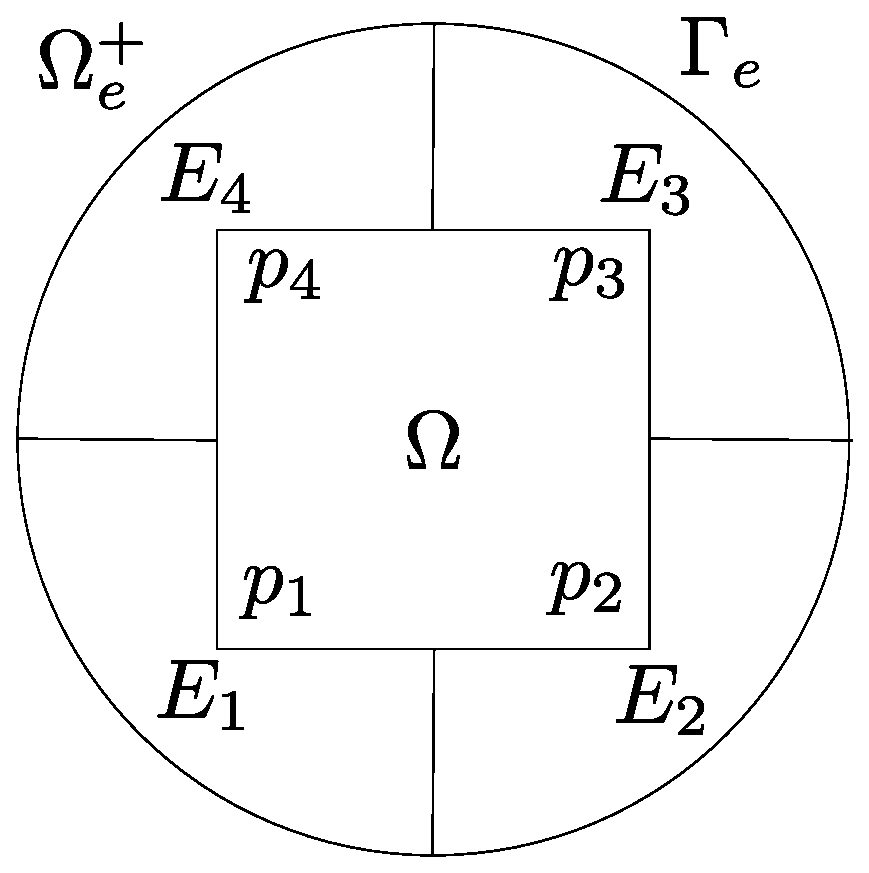
\includegraphics[width=6cm]{geometry}
\vspace{-.5cm}
\label{fig:geom}
\end{figure}


To achieve high accuracy we cannot simply use fundamental soluitions
to approximate the scattered field. The problem is the singularities
of the solution $u$ at the corners. If these are not represented in
the basis our approximation error will decay very slowly as the number
of basis functions increases. To solve this problem we use the domain
decompositon shown in Figure \ref{fig:geom}. The idea is that each of
the elements $E_i$ only contains one corner $p_i$ of the square. We can then
match the corner behavior in each domain by using fractional order
Bessel functions. Since furthermore, $u=0$ on $\partial\Omega$ it will
be sufficient to use Fourier-Bessel sine functions that automatically
satisfy the zero boundary conditions on the sides of the square.
Hence, the total field $u$ is approximated in each element $E_i$ using
an approximation of the form
$$
u(r,\theta)\approx
\sum_{j=1}^{N_i}c_j^{(i)}J_{\frac{2}{3}j}(kr)\sin(\frac{2j}{3}\theta).
$$
The polar coordinate system in each element $E_i$ is rotated in such a way
that the basis functions are zero on the sides adjacent to the corner
at $p_i$.

In the infinite domain $\Omega_e^+$ we use a basis of fundamental
solutions to represent the scattered field $u_s$. Hence, for
$\bx\in\Omega^+$ we have
$$
u_s(\bx)\approx \sum_{j=1}^{N_e}\frac{i}{4}c_j^{(e)}H_0^{(1)}(|\bx-\by_j|),
$$
where $\by_j=r_{mfs}e^{i\phi_j}$ and $\phi_j=\frac{2\pi j}{N_e}$. Note
that we approximate with the fundamental solutions the scattered field
$u_s$ while in the finite subdomains $E_i$ we approximate the total
field $u$. The compatibility conditions between approximations $u^{i}$
und $u^{j}$ in two neighboring elements $E_i$ and $E_j$ with common
boundary $\Gamma_{ij}$ are given by
$$
u^{(i)}(\bx)\approx u^{(j)}(\bx),\quad \frac{\partial u}{\partial
  n_i}{u^{(i)}}(\bx)\approx  \frac{\partial u}{\partial
  n_i}{u^{(j)}}(\bx),
$$
where $\bx\in\Gamma_{ij}$ and $\frac{\partial}{\partial\nu_i}$ is the
outward normal derivative at the boundary of $E_i$.
On the interface $\Gamma_{ie}$ between an element $E_i$ and the
exterior domain $\Omega_e^{+}$ we have the compatibility conditions
$$
u^{(i)}(\bx)\approx u_{inc}(\bx)+u_s^{(e)}(\bx),\quad \frac{\partial}{\partial
  n_i}{u^{(i)}}(\bx)\approx  \frac{\partial}{\partial
  n_i}{(u_s^{(e)}+u_{inc})}(\bx),
$$
where $u_s^{(i)}$ is the fundamental solutions approximation to the
scattered field in $\Omega_e^{+}$. We have to add the incident field
to the approximate scattered field since we are matching with the
total field in the elements $E_i$.
An approximate solution to the whole problem is now 
computed by minimizing the $L^2$ error of 
the compatibility conditions on all interfaces.

\subsubsection{Implementation in \mpspack}

Although the setup of the problem seems quite complicated we will see
that it is very simple to set it up in \mpspack. Indeed, the most part
of the code will be devoted to creating the mesh structure from
Figure \ref{fig:geom}.

\paragraph{Initialization of the problem parameters}

We need to define the following problem parameters.
\begin{verbatim}
k = 50;      % Wavenumber
r = 1.0;     % Radius of outer circle    
M = 200;     % Number of quadrature points on segments
N=100;       % Number of basis fct. in each subdomain
a=.5;        % Half-Size of the square
rmfs=0.8*r;  % Radius of the fundamental solutions curve
\end{verbatim}


\paragraph{Setup of the geometry}

We now need to define the geometry. Fortunately,
\mpspack gives some support for the construction of the geometry.

First we define the segments of one element ($E_3$ in Figure
\ref{fig:geom}). This is done with the following three commands.

\begin{verbatim}
s = segment.polyseglist(M, [1i*r 1i*a a+1i*a a r], 'g');
s=[s(1:3) segment(2*M, [0 r 0 pi/2])];
s = [s rotate(s, pi/2) rotate(s, pi) rotate(s, 3*pi/2)];
\end{verbatim}
The first command defines all the straight lines that form part of the
boundary of $E_3$. For this we use {\texttt{polyseglist}}. The command
{\texttt polyseglist} constructs a closed polygon. We then delete the
last two segments of the array {\texttt s} and add instead the
circular line segment. This results in the segments shown in the left
plot of Figure \ref{fig:elem1}. We now rotate this element three times to
obtain the segments showin in the right plot of Figure \ref{fig:circelem}.
\begin{figure}
\begin{tabular}{cc}
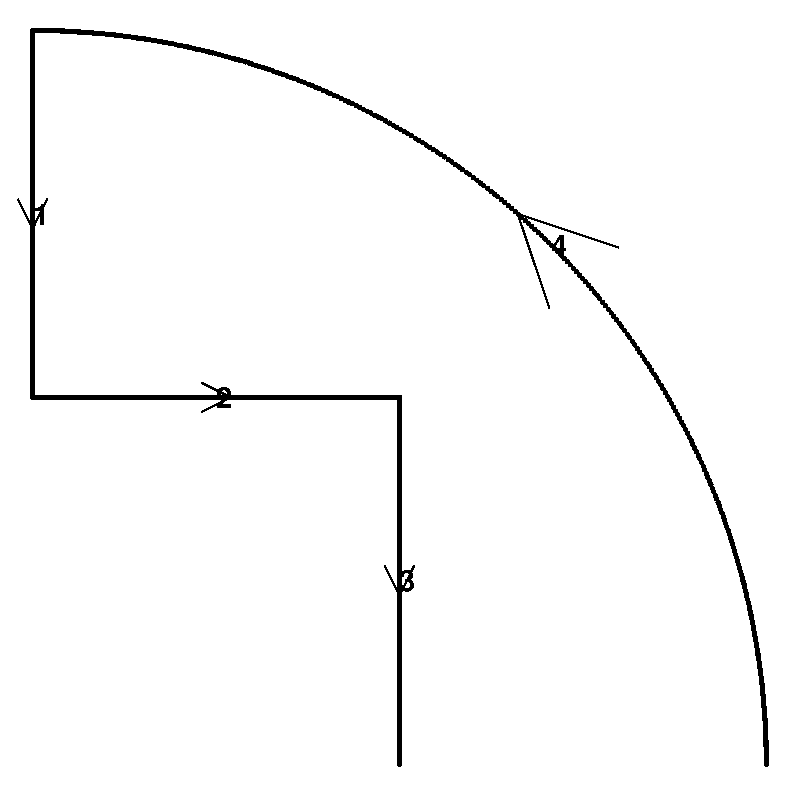
\includegraphics[width=5cm]{circelem1} &
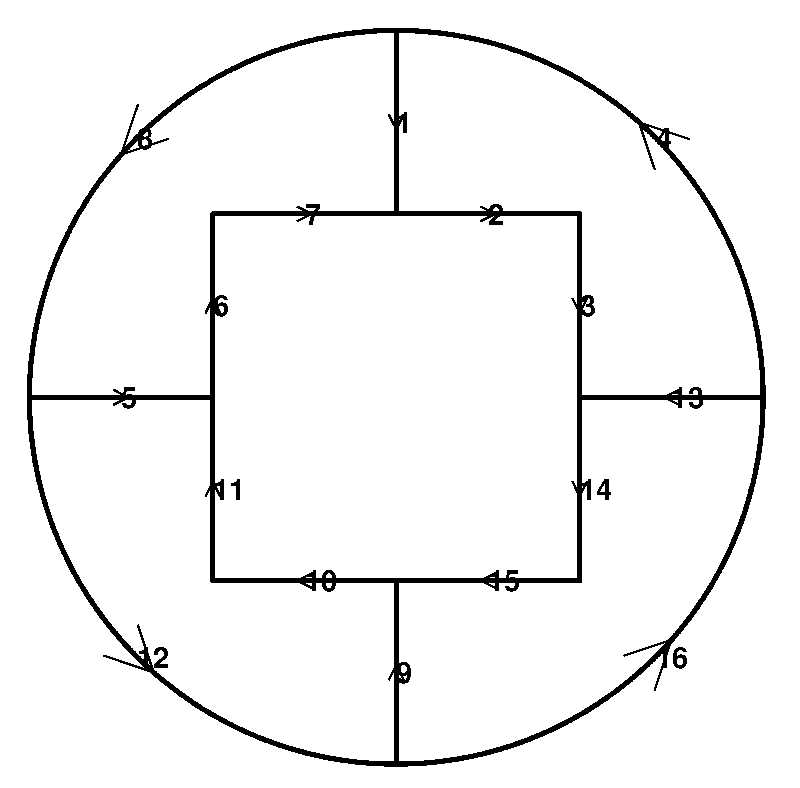
\includegraphics[width=5cm]{circelem2}
\end{tabular}
\caption{The segments in the right plot are created by rotating the segments
  shown in the left plot.}
\label{fig:circelem}
\end{figure}

For later it is important to have a separate list of all segments not
belonging to the square and all segments belonging to the outer
circle.

\begin{verbatim}
sdecomp=s([1 4 5 8 9 12 13 16]); % All artificial boundaries
extlist=s([4 8 12 16]);          % Segments forming the outer circle
\end{verbatim}

We now define the domains. To make the code shorter and use a simple
for loop we can use the rotational symmetry of the segments in this
problem.

\begin{verbatim}
d=domain.empty(4,0);
for j=1:4, d(j)=domain(s(1+mod(4*(j-1)+[0 1 2 12 3],16)),[1 1 1 -1 1]); end
ext = domain([], [],extlist(end:-1:1), -1); 
\end{verbatim}
The for loop looks slightly complicated. But all it does is pick out
the right indices for the elements forming a domain and creating it
together with the right sense of direction. At the end we have an
array {\texttt d} containing the four fine domains $E_i$. The exterior
domain {\texttt ext} is created by traversing {\texttt extlist} in
reverse order with reversed sense $-1$. This is necessary since we now
have the boundary of an exterior domain, which has a reversed sense of
direction.

Setting up the compatibility conditions is now trivial. It is done by
the command
\begin{verbatim}
sdecomp.setmatch([k -k],[1 -1]);
\end{verbatim}
The matching conditions for the function values are scaled by the
wavenumber $k$ to balance the different scaling between the $L^2$ error
in the function and the $L^2$ error in the
derivative.\footnote{Consider the one dimensional plane wave
  $e^{ikx}$. The derivative is $ike^{ikx}$. Hence, in general it makes sense to
  scale the $L^2$ error of function values by $k$ to give it the same
  dimension as the $L^2$ error of the derivative.}

We can now add the basis functions to the domains. This is done by the
following two commands.




%%% Local Variables: 
%%% mode: latex
%%% TeX-master: "tutorial"
%%% End: 


\bibliographystyle{siam} 
\bibliography{alexrefs}
\end{document}
